\documentclass[12pt,a4paper]{article}
\usepackage[T1]{fontenc}         
\usepackage[utf8]{inputenc}      
\usepackage{lmodern}             
\usepackage[margin=2.5cm]{geometry}
\usepackage{graphicx}
\usepackage{booktabs}
%\usepackage{hyperref}
\usepackage{caption}
\usepackage{subcaption}
\usepackage{tikz}
\usetikzlibrary{shapes.geometric, arrows, positioning, calc}
\usepackage{pgfplots}
\pgfplotsset{compat=1.18}


\title{Continuous Model of Human Behavior Based on Constitutional Axis and Nasion Acupoint Polarity:\\
Social Groups, Intimate Relationships, Family, and Extreme Situations}

\author{
DuckJin Yoon (Solvaram)\\
Eight-Constitutional Research Platform
}

\date{\today}
\usepackage[hidelinks]{hyperref}
\begin{document}

\maketitle

\begin{abstract}
This study analyzes human social interactions, intimate relationships, and behaviors under extreme conditions using a continuous, instinctive bio-mechanical framework based on the Constitutional Axis and Nasion Acupoint Polarity \cite{Yoon2026a,Yoon2026b}. Observations indicate that in general groups, individuals sharing the same axis and polarity naturally cluster, while those of the same axis but opposite polarity partially join, creating loose but repeated instinctive diffusion patterns \cite{Yoon2026c}. In intimate relationships, shared Nasion acupoint with opposite polarity induces instinctive attraction and cooperative restraint, whereas within families, sequential polarity of children strengthens parent-child relationship stability \cite{Yoon2026a}. In extreme situations, lateral personnel and the subject align on the same axis but opposite polarity, enhancing behavior predictability and control \cite{Yoon2026b}. These repeated patterns demonstrate natural inevitability rather than coincidence \cite{Yoon2026c}.
\end{abstract}

\tableofcontents

\vspace{2cm} % 1cm의 수직 공간 추가

\section{Introduction}
\subsection{Background}
In general groups such as students and military personnel, individuals of the same axis and polarity constitute approximately 80\% of clusters \cite{Yoon2026c}. Those of the same axis but opposite polarity make up about 15\%, forming loose but repeated instinctive diffusion patterns \cite{Yoon2026c}.  

In intimate or marital relationships, same Nasion acupoint with opposite polarity produces instinctive attraction and cooperative restraint \cite{Yoon2026a}. Same polarity combinations maintain friendship and stability \cite{Yoon2026a}. Within families, children with sequential opposite polarity naturally strengthen intimacy and stability \cite{Yoon2026a}.  

In extreme situations (e.g., investigation, apprehension), lateral personnel and the subject are positioned with same axis but opposite polarity, maximizing predictability and behavioral control \cite{Yoon2026b}.

\subsection{Objectives}
\begin{enumerate}
\item Quantify continuous human behavior patterns based on Constitutional Axis and Nasion Acupoint Polarity \cite{Yoon2026a}.
\item Present behavioral prediction models for general groups, intimate relationships, family, and extreme situations \cite{Yoon2026b}.
\item Demonstrate natural linkage between instinctive stability and social behavior \cite{Yoon2026c}.
\end{enumerate}

\subsection{Scientific Contribution}
This study provides the first application of Constitutional Axis-based behavioral models across social and extreme environments, explaining instinctive stability and cooperative mechanisms in a continuous natural framework \cite{Yoon2026a,Yoon2026b}.

\section{Methods}
\subsection{Subjects}
Students, military personnel, general groups, intimate/marital relationships, families, and extreme scenarios included \cite{Yoon2026c}.

\subsection{Detection Tools}
BIMOD and Nasion acupoint-based axis/polarity discrimination \cite{Yoon2026a}.

\subsection{Analysis Metrics}
Axis homogeneity, polarity match \& opposite, group composition ratio, predictability, friendship \& cooperation levels \cite{Yoon2026b}.

\section{Results}
\subsection{General Groups}
Same axis \& same polarity 1st cluster 80\% \cite{Yoon2026c} \\
Same axis \& opposite polarity 2nd cluster 15\% \cite{Yoon2026c}

\subsection{Intimate/Marital Relationships}
Same axis \& opposite polarity instinctive attraction, cooperative restraint \cite{Yoon2026a} \\
Same axis \& same polarity friendship maintenance \cite{Yoon2026a}

\subsection{Family/Children}
Sequential child polarity enhanced parent-child stability \cite{Yoon2026a}

\subsection{Extreme Situations}
In extreme situations, alignment on the same axis with opposite polarity between bilaterally positioned investigative officers and the subject constitutes a structural condition that necessarily produces predictable and controllable behavior. \cite{Yoon2026b}

\section{Discussion}
Results show that repeated human behavior patterns are naturally inevitable \cite{Yoon2026c}. Same axis \& same polarity friendship and stability; opposite polarity instinctive attraction and cooperative restraint \cite{Yoon2026a}. Continuous model demonstrates predictable social stability based on Constitutional Axis \cite{Yoon2026b}.

\section{Conclusion}
We propose a human behavior model based on Constitutional Axis and Nasion Acupoint Polarity. Instinctive perception and psychological stability enable repeated behavior prediction in general groups, intimate relationships, families, and extreme scenarios \cite{Yoon2026a,Yoon2026b,Yoon2026c}.

\clearpage

\section{Figures and Matrices}
\begin{figure}[ht]
\centering
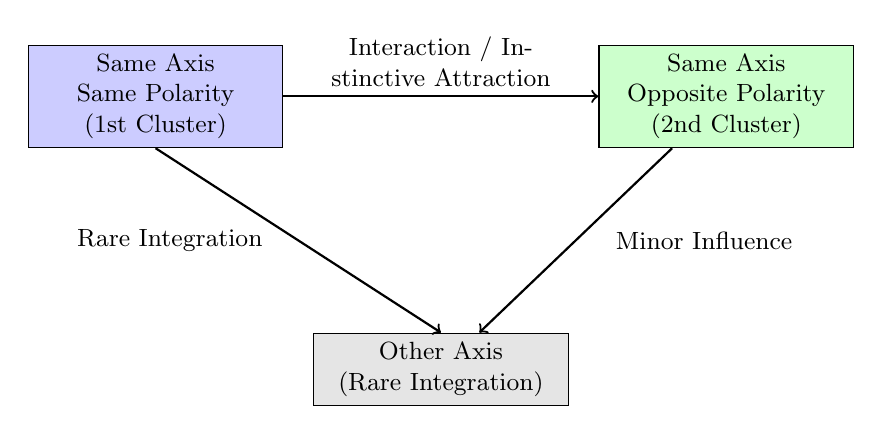
\begin{tikzpicture}[node distance=2cm, every node/.style={font=\small, align=center, text width=3cm}]
\node (sameAxisSamePol) [rectangle, draw, fill=blue!20] {Same Axis \\ Same Polarity \\ (1st Cluster)};
\node (sameAxisOppPol) [rectangle, draw, fill=green!20, right=4cm of sameAxisSamePol] {Same Axis \\ Opposite Polarity \\ (2nd Cluster)};
\node (otherAxis) [rectangle, draw, fill=gray!20, below=3cm of $(sameAxisSamePol)!0.5!(sameAxisOppPol)$] {Other Axis \\ (Rare Integration)};

\draw[->, thick] (sameAxisSamePol) -- (sameAxisOppPol) node[midway, above] {Interaction / Instinctive Attraction};
\draw[->, thick] (sameAxisOppPol) -- (otherAxis) node[midway, right] {Minor Influence};
\draw[->, thick] (sameAxisSamePol.south) -- (otherAxis.north) node[midway, left] {Rare Integration};
\end{tikzpicture}
\caption{Behavior Prediction Matrix Based on Constitutional Axis and Polarity}
\end{figure}

\begin{figure}[ht]
\centering
\resizebox{\textwidth}{!}{
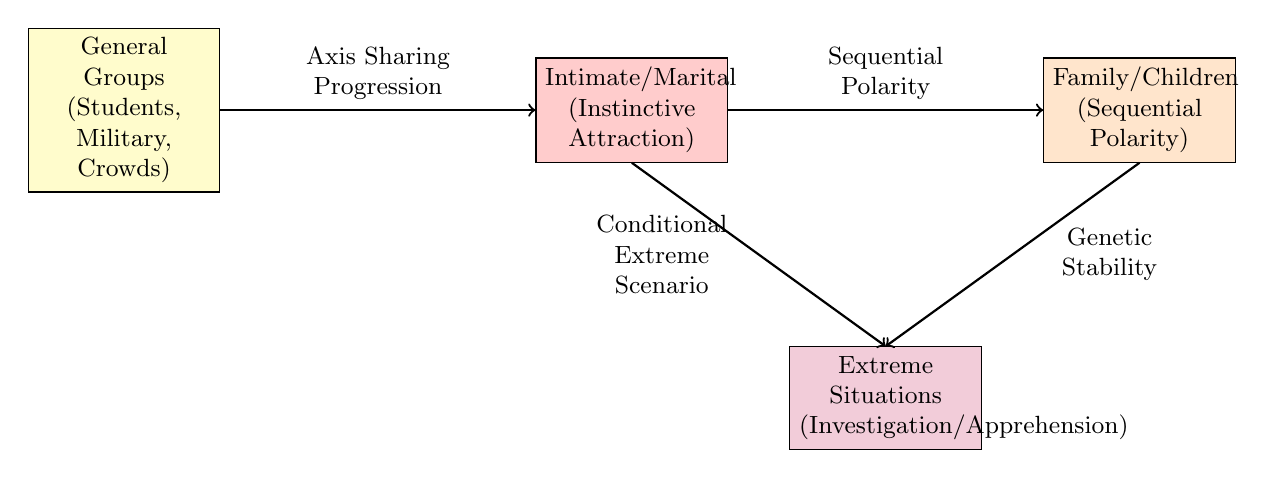
\begin{tikzpicture}[scale=0.9, node distance=3cm, every node/.style={font=\small, align=center, text width=2.2cm}]
\node (general) [rectangle, draw, fill=yellow!20] {General Groups \\ (Students, Military, Crowds)};
\node (romantic) [rectangle, draw, fill=red!20, right=4cm of general] {Intimate/Marital \\ (Instinctive Attraction)};
\node (family) [rectangle, draw, fill=orange!20, right=4cm of romantic] {Family/Children \\ (Sequential Polarity)};
\node (extreme) [rectangle, draw, fill=purple!20, below=3cm of $(romantic)!0.5!(family)$] {Extreme Situations \\ (Investigation/Apprehension)};

\draw[->, thick] (general) -- (romantic) node[midway, above] {Axis Sharing Progression};
\draw[->, thick] (romantic) -- (family) node[midway, above] {Sequential Polarity};
\draw[->, thick] (romantic.south) -- (extreme.north) node[midway, left] {Conditional Extreme Scenario};
\draw[->, thick] (family.south) -- (extreme.north) node[midway, right] {Genetic Stability};
\end{tikzpicture}

}

\caption{Continuous Flow Across Groups, Intimate Relationships, Family, and Extreme Situations}
\end{figure}

\bibliographystyle{plain}
\bibliography{BIMOD_300_references}

\end{document}
